\section{Online feliratok letöltése}

Az alkalmazást a kényelmesebb és felhasználóbarátabb használatért kiegészítettem egy, az alapspecifikáción kívül eső funkcióval, mely az online feliratok keresése és letöltése. Habár korlátlan mennyiségű felirat áll rendelkezésre online, a felhasználók egy része mégsem ismeri ezek beszerzésének módjait. Legfőképpen nekik nyújthat nagy segítséget az implementált funkció, azonban mindenki számára egy kényelmes megoldást kínál. A megvalósításhoz az egyik legnagyobb felirat-adatbázissal rendelkező weboldal saját \textit{API}-ját, az \textit{opensub4j} nevű interfészt hívtam segítségül. A weboldalon történő ingyenes regisztráció után mar használhattam is a felületet.

Első lépésként felvettem egy új függőséget az alkalmazás \textit{pom} fájljába. Ettől kezdve elérhetővé váltak számomra a csomagban definiált osztályok. A funkció implementálását a \textit{SRTSearchFrame.java} osztály tartalmazza. Működése két részből áll: a feliratok keresése, illetve ezek letöltése, kitömörítése.

\subsection{Feliratok keresése}

\begin{figure}[h!]
  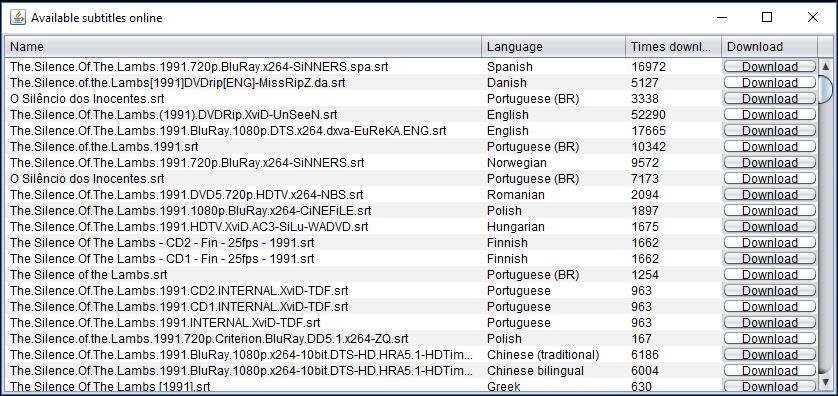
\includegraphics[width=\linewidth]{images/online_search.jpg}
  \caption{Keresési találatokat tartalmazó táblázat}
  \label{fig:online_search}
\end{figure}

A keresőpanel megjeleníthető az alkalmazás alsó kezelőfelületén a \textit{Search for subtitles online} gombra történő kattintással. Ekkor egy egyszerű felület tárul a felhasználó elé. Itt választhat, hogy filmhez, vagy sorozathoz készült feliratot keres. A kettőt azért volt szükséges szétválasztani, mert a két kérés címe mindkét esetben más. A keresési módok között a bal oldalon lévő \textit{JToggleButton}-ra történő kattintással van lehetőség váltásra. Filmek esetében csak a címet, sorozatok esetében pedig a címet, illetve lehetőség szerint az évadot, epizódot kell megadnunk. A \textit{Search} gombra történő kattintással elindíthatjuk a keresést, melyet az alábbi függvény végez (\ref{lst:search}). A keresés nyelvét egy rendszerváltozóból kapja, a név-évad-epizód hármast pedig a megfelelő \textit{JTextField}-ekből. Ezután a \textit{.srt} kiterjesztésre való szűrés megy végbe. 

\begin{spacing}{1.25}
\begin{lstlisting}[caption=Feliratok keresése sorozatokhoz valamint filmekhez, label={lst:search}, language=java]
//if it is a serial
if (isSerial.isSelected()) {
    subtitles = osClient.searchSubtitles(
    System.getProperty("user.language"),
    nameTextField.getText(),
    seasonTextField.getText(),
    episodeTextField.getText())
        .stream()
        .filter(sub -> sub.getFormat()
        .equals("srt"))
        .collect(Collectors.toList());
//if it is a movie
} else {
    //...
}
\end{lstlisting}
\end{spacing}

A művelethez természetesen internetkapcsolat szükséges, ennek hiányában az alkalmazás hibaüzenetet jelenít meg a felhasználónak, az \textit{An unexpected error has occurred. Please check your internet connection.} szöveggel. Mivel az \textit{API} képes kezelni a hiányos, esetleg hibás keresési feltéteket, így legtöbbször elég a film vagy sorozat címének egy részét is megadni. Amennyiben a keresés sikeres egy táblázat tárul elénk (\ref{fig:online_search}), amely az összes megtalált felirat közül -az alkalmazás kompatibilitása miatt-, csak a \textit{.srt} kiterjesztésűeket tartalmazza. A táblázatban megjelenik a feliratfájl neve, nyelve, letöltéseinek száma, valamint egy \textit{Download} gomb, mely a felirat letöltését indítja el.

\subsection{Feliratok letöltése}

\begin{spacing}{1.25}
\begin{figure}
  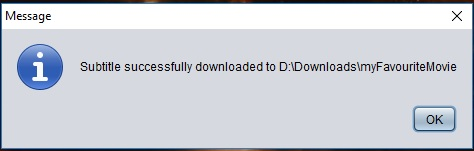
\includegraphics[width=\linewidth]{images/downloaded_sub.jpg}
  \caption{A letöltés helyét megjelenítő információs panel}
  \label{fig:downloaded_sub}
\end{figure}
\end{spacing}

Miután megtaláltuk a számunkra megfelelő feliratot, kattintsunk a letöltés gombra. Sikeres letöltés esetén egy \textit{JOptionPane} jelenik meg a képernyőn, amely tájékoztatja a felhasználót a letöltött fájlt tartalmazó könyvtárról (\ref{fig:downloaded_sub}). Ez alapértelmezetten a \textit{user.dir} rendszerváltozóból kerül kiolvasásra, azonban amennyiben bármilyen médiafájl már importálásra került a lejátszóba, a letöltés annak a fájlnak a tartalmazó könyvtárába kerül (). A letöltést a \textit{Wget.java} osztály végzi, amely egyetlen metódust tartalmaz. Ez paraméterként a mentendő fájl URL-jét, valamint egy útvonalat vár, ahova a kiírás történik. Törzsében egy \textit{HttpURLConnection}-ön keresztül egy \textit{GET} kérést indít, amely \textit{InputStream}-ként adja át az adatokat. Mivel az állomány tömörített, ezért \textit{ArchiveInputStream} használatára is szükség van, amely a \textit{stream}-et megfelelően kezeli. A metódus létrehoz egy \textit{OutputStream}-et, amelybe átkonvertálja az \textit{InputStream} tartalmát. Végül mindkét \textit{stream}-et lezárja. E folyamat segítségével az alkalmazás képes a letöltött állományt kitömörítve elmenteni a felhasználó merevlemezére, amely így már azonnal importálható a lejátszóba.